% Baccalauréat malgache, série C, 2010 : corrigé.
\TCDBacAttribution{C}{2010}
\providecommand{\cm}{~\mathrm{cm}}
\providecommand{\Plan}{(\mathscr{P})}
\providecommand{\dx}{~\mathrm{d}x}
\providecommand{\dt}{\mathrm{d}t}
\providecommand{\Ouv}{(O;\vec{u},\vec{v})}
\providecommand{\mes}[2]{\mathrm{mes}\left( \widehat{ \overrightarrow{#1} ; \overrightarrow{#2} } \right)}
\providecommand{\D}{(\mathscr{D})}
\providecommand{\Courbe}{(\mathscr{C})}
\providecommand{\Courben}{(\mathscr{C}_n)}
\providecommand{\CourbeU}{(\mathscr{C}_1)}
\providecommand{\CourbeD}{(\mathscr{C}_2)}
\providecommand{\bary}[1]{\mathrm{bar}\left\lbrace #1 \right\rbrace}
\providecommand{\congru}[3]{#1 \equiv #2 \quad \left[ \mathrm{mod}~#3\right]}
\providecommand{\Angl}[2]{\left( \widehat{ \overrightarrow{#1} , \overrightarrow{#2} } \right)}
%
%%%%%%%%%%%%%%%%%%%%%%%%%%%%%%%%%%%%%%%%%%%%%%%%%%%%%%%%%%%%%%%%%%%%%%%%%%%%%%%%%%%%%%%%%%%%%%%%%%%%%%%%%%%%%%%%%%%%%%%%%%%%%%%%
\noindent \underline{\textsc{\textbf{Exercice}}} (4 points)
\begin{description}
	\item[A- Arithmétique.]
	\begin{enumerate}
		\item \vln{Division euclidienne de $-283$ par $19$ :}
			$19 \times 15 = 285$, donc $-283 = -285 + 2 = 19 \times (-15) + 2$ avec $0 \leq 2 < 19$.
			\par\noindent\ansbox{$-283 = 19 \times (-15) + 2$ : quotient $-15$, reste $2$.}
		\item
		\begin{enumerate}
			\item \vln{Congruence :}
				$11 = 7 \times 1 + 4$, donc \par\noindent\ansbox{$11 \equiv 4 \pmod 7$.}
			\item \vln{Divisibilité par $7$ :}
				$2^3 = 8 \equiv 1 \pmod 7$, donc $2^{3n+1} = 2 \times 8^n \equiv 2$.
				$3^6 = 729 = 7 \times 104 + 1 \equiv 1 \pmod 7$, donc $3^{6n} \equiv 1$.
				$11^{3n+1} \equiv 4^{3n+1} = 4 \times 64^n$ et $64 = 7 \times 9 + 1 \equiv 1$, donc $11^{3n+1} \equiv 4$.
				Ainsi $2^{3n+1} + 3^{6n} + 11^{3n+1} \equiv 2 + 1 + 4 = 7 \equiv 0 \pmod 7$.
				\par\noindent\ansbox{Pour tout $n \in \mathbb{N}$, $7$ divise $2^{3n+1} + 3^{6n} + 11^{3n+1}$.}
		\end{enumerate}
		\item \vln{Critère de divisibilité par $11$ :}
			$X = \sum_{i=0}^{p} a_i 10^i$ et $10 \equiv -1 \pmod{11}$, donc $10^i \equiv (-1)^i$ et
			$X \equiv \sum_{i=0}^{p} (-1)^i a_i \pmod{11}$.
			\par\noindent\ansbox{Si $\sum_{i=0}^{p} (-1)^i a_i \equiv 0 \pmod{11}$, alors $X \equiv 0 \pmod{11}$}
			(et réciproquement).
	\end{enumerate}
	\item[B- Probabilité.]
	Un menu est un triplet (entrée, plat, dessert) : $3 \times 5 \times 4 = 60$ menus, choisis au hasard donc équiprobables.
	\begin{enumerate}
		\item \vln{Poisson frit :}
			$3 \times 1 \times 4 = 12$ menus contiennent le poisson frit : $P = \frac{12}{60}$, soit \par\noindent\ansbox{$P = \frac{1}{5}$.}
		\item \vln{Crudité et glace aux fraises :}
			$2 \times 5 \times 1 = 10$ menus : $P = \frac{10}{60}$, soit \par\noindent\ansbox{$P = \frac{1}{6}$.}
		\item \vln{Crudité, poisson frit et glace aux fraises :}
			$2 \times 1 \times 1 = 2$ menus : $P = \frac{2}{60}$, soit \par\noindent\ansbox{$P = \frac{1}{30}$.}
	\end{enumerate}
\end{description}
%%%%%%%%%%%%%%%%%%%%%%%%%%%%%%%%%%%%%%%%%%%%%%%%%%%%%%%%%%%%%%%%%%%%%%%%%%%%%%%%%%%%%%%%%%%%%%%%%%%%%%%%%%%%%%%%%%%%%%%%%%%%%%%%
\noindent \underline{\textsc{\textbf{PROBLEME I}}} (7 points)
\begin{description}
	\item[Partie A]
	\vln{Centre de $r_1 \circ r_2$ :}
	Le triangle $TED$ est équilatéral direct, donc ses angles orientés valent $\frac{\pi}{3}$ : $\left((DT),(DE)\right) = \frac{\pi}{3}$ et $\left((ED),(ET)\right) = \frac{\pi}{3}$ (angles de droites, modulo $\pi$).
	Par le théorème de décomposition :
	$r_2 = s_{(DE)} \circ s_{(DT)}$ (centre $D$, angle $2 \times \frac{\pi}{3}$) et $r_1 = s_{(ET)} \circ s_{(ED)}$ (centre $E$, angle $2 \times \frac{\pi}{3}$).
	Donc $r_1 \circ r_2 = s_{(ET)} \circ s_{(ED)} \circ s_{(DE)} \circ s_{(DT)} = s_{(ET)} \circ s_{(DT)}$.
	Les droites $(DT)$ et $(ET)$ se coupent en $T$ et $2\left((DT),(ET)\right) = 2\left(\frac{\pi}{3} + \frac{\pi}{3}\right) = \frac{4\pi}{3}$.
	\par\noindent\ansbox{$r_1 \circ r_2$ est la rotation de centre $T$ et d'angle $\frac{4\pi}{3}$ (soit $-\frac{2\pi}{3}$).}
	\item[Partie B]
	\begin{enumerate}
		\item \vln{Construction :}
			Le parallélogramme $OJKL$ dépend du choix de $L$ (l'énoncé ne le fixe pas) ; $P$ est l'image de $L$ par la rotation $r$ de centre $O$ et d'angle $\frac{\pi}{3}$.
			Exemple de figure :
			\begin{center}
			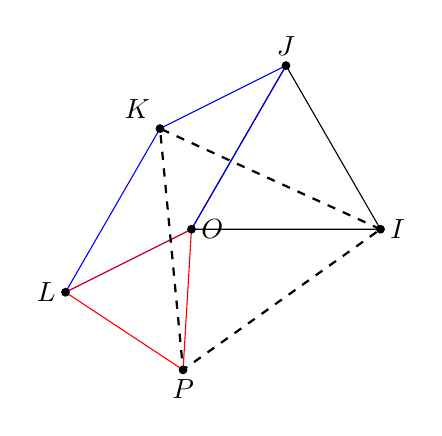
\begin{tikzpicture}[scale=.8]
				\coordinate (O) at (0,0); \coordinate (I) at (3,0); \coordinate (J) at (1.5,2.598);
				\coordinate (L) at (-2,-1); \coordinate (K) at (-0.5,1.598); \coordinate (P) at (-0.134,-2.232);
				\draw (O) -- (I) -- (J) -- cycle;
				\draw[blue] (O) -- (J) -- (K) -- (L) -- cycle;
				\draw[red] (O) -- (L) -- (P) -- cycle;
				\draw[dashed,thick] (I) -- (K) -- (P) -- cycle;
				\foreach \P/\pos in {O/right,I/right,J/above,K/above left,L/left,P/below}
					\fill (\P) circle (2pt) node[\pos] {$\P$};
			\end{tikzpicture}
			\end{center}
		\item
		\begin{enumerate}
			\item \vln{Nature de $g = r \circ t$ :}
				Une translation est un déplacement d'angle $0$ ; $g$ est donc un déplacement d'angle $0 + \frac{\pi}{3} = \frac{\pi}{3} \neq 0$.
				\par\noindent\ansbox{$g$ est une rotation d'angle $\frac{\pi}{3}$.}
			\item \vln{Images de $I$ et de $K$ :}
				$t(I) = I_1$ avec $\overrightarrow{II_1} = \overrightarrow{JO}$, donc $\overrightarrow{OI_1} = \overrightarrow{JI}$.
				Le triangle $OIJ$ étant équilatéral direct, la rotation $r$ transforme $\overrightarrow{JI}$ en $\overrightarrow{OI}$
				(car $\Angl{JI}{OI} = \frac{\pi}{3}$ et $JI = OI$) ; donc $r(I_1) = I$ : \par\noindent\ansbox{$g(I) = I$.}
				$t(K) = K_1$ avec $\overrightarrow{OK_1} = \overrightarrow{JK} = \overrightarrow{OL}$ (parallélogramme $OJKL$), donc $K_1 = L$, et $r(L) = P$ ($OLP$ équilatéral direct).
				\par\noindent\ansbox{$g(K) = P$.}
				$g$ est une rotation d'angle $\frac{\pi}{3}$ qui fixe $I$ :
				\par\noindent\ansbox{$g$ est la rotation de centre $I$ et d'angle $\frac{\pi}{3}$.}
				Comme $g(K) = P$ : $IK = IP$ et $\Angl{IK}{IP} = \frac{\pi}{3}$.
				\par\noindent\ansbox{Le triangle $IKP$ est équilatéral direct.}
		\end{enumerate}
	\end{enumerate}
	\item[Partie C]
	\begin{description}
		\item[I.]
		\begin{enumerate}
			\item \vln{$(EQ)$ et $(NR)$ passent par $H$ :}
				Par associativité du barycentre, $H = \bary{(M,3);(E,1);(N,1)} = \bary{(Q,4);(E,1)}$ car $Q = \bary{(M,3);(N,1)}$.
				Donc $H \in (EQ)$. De même $H = \bary{(R,4);(N,1)}$, donc $H \in (NR)$.
				\par\noindent\ansbox{Les droites $(EQ)$ et $(NR)$ passent par $H$.}
			\item
			\begin{enumerate}
				\item \vln{Alignement de $M$, $P$, $H$ :}
					$P = \bary{(E,1);(N,1)}$, donc $H = \bary{(M,3);(P,2)}$ : \par\noindent\ansbox{$M$, $P$, $H$ sont alignés.}
				\item \vln{$\overrightarrow{PH}$ en fonction de $\overrightarrow{PM}$ :}
					$\overrightarrow{PH} = \frac{3\overrightarrow{PM} + 2\overrightarrow{PP}}{5}$, d'où \par\noindent\ansbox{$\overrightarrow{PH} = \frac{3}{5}\overrightarrow{PM}$.}
			\end{enumerate}
		\end{enumerate}
		\item[II.]
		\begin{enumerate}
			\item \vln{Point $G$ :}
				La somme des poids est $4 - 1 - 1 = 2 \neq 0$, et
				$\overrightarrow{AG} = \frac{-\overrightarrow{AB} - \overrightarrow{AC}}{2} = -\overrightarrow{AI}$ où $I$ est le milieu de $[BC]$.
				\par\noindent\ansbox{$G$ est le symétrique du milieu $I$ de $[BC]$ par rapport à $A$.}
				On a $AG = AI = \frac{a\sqrt{2}}{2}$ : $G$ est sur la médiatrice de $[BC]$, de l'autre côté de $A$ par rapport à $I$.
			\item \vln{Ensemble $(\mathscr{E})$ :}
				Relation de Leibniz : $4MA^2 - MB^2 - MC^2 = 2MG^2 + 4GA^2 - GB^2 - GC^2$.
				$GA^2 = \frac{a^2}{2}$ ; $(GA) \perp (BC)$ et $GI = 2AI = a\sqrt{2}$, $IB = \frac{a\sqrt{2}}{2}$, donc $GB^2 = GC^2 = 2a^2 + \frac{a^2}{2} = \frac{5a^2}{2}$.
				La constante vaut $2a^2 - 5a^2 = -3a^2$ et la condition s'écrit $2MG^2 - 3a^2 = 2a^2$, soit $MG^2 = \frac{5a^2}{2}$.
				\par\noindent\ansbox{$(\mathscr{E})$ est le cercle de centre $G$ et de rayon $\frac{a\sqrt{10}}{2}$.}
				Comme $GB = GC = \frac{a\sqrt{10}}{2}$, ce cercle passe par $B$ et $C$ : on le construit comme le cercle de centre $G$ passant par $B$.
				\begin{center}
				\begin{tikzpicture}[scale=.8]
					\coordinate (A) at (0,0); \coordinate (B) at (3,0); \coordinate (C) at (0,3);
					\coordinate (I) at (1.5,1.5); \coordinate (G) at (-1.5,-1.5);
					\draw (A) -- (B) -- (C) -- cycle;
					\draw[dashed] (G) -- (I);
					\draw[blue] (G) circle (4.743);
					\foreach \P/\pos in {A/below left,B/below right,C/above left,I/above right,G/below left}
						\fill (\P) circle (2pt) node[\pos] {$\P$};
					\node[blue] at (2.6,2.6) {$(\mathscr{E})$};
				\end{tikzpicture}
				\end{center}
		\end{enumerate}
	\end{description}
\end{description}
%%%%%%%%%%%%%%%%%%%%%%%%%%%%%%%%%%%%%%%%%%%%%%%%%%%%%%%%%%%%%%%%%%%%%%%%%%%%%%%%%%%%%%%%%%%%%%%%%%%%%%%%%%%%%%%%%%%%%%%%%%%%%%%%
\noindent \underline{\textsc{\textbf{PROBLEME II}}} (9 points)
\begin{description}
	\item[PARTIE I]
	\begin{description}
		\item[A. ]
		\begin{enumerate}
			\item \vln{Ensemble de définition :}
				Pour $0 < x < 1$, $\ln x \neq 0$ ; $f$ est aussi définie en $0$ et en $1$ par les valeurs données.
				\par\noindent\ansbox{$D_f = [0 ; 1]$.}
			\item \vln{Continuité en $0$ et en $1$ :}
				En $0^+$ : $x - 1 \to -1$ et $\ln x \to -\infty$, donc $f(x) \to 0 = f(0)$.
				En $1^-$ : $\frac{\ln x}{x - 1} = \frac{\ln x - \ln 1}{x - 1} \to (\ln)'(1) = 1$, donc $f(x) \to 1 = f(1)$.
				\par\noindent\ansbox{$f$ est continue (à droite) en $0$ et (à gauche) en $1$.}
			\item \vln{Dérivabilité sur $]0;1[$ et signe de $f'$ :}
				Sur $]0;1[$, $f$ est le quotient de deux fonctions dérivables, le dénominateur ne s'annulant pas : $f$ est dérivable et
				\[
					f'(x) = \frac{\ln x - (x-1)\frac{1}{x}}{(\ln x)^2} = \frac{\ln x - 1 + \frac{1}{x}}{(\ln x)^2} = \frac{H(x)}{(\ln x)^2} .
				\]
				\par\noindent\ansbox{$(\ln x)^2 > 0$ : $f'(x)$ a le signe de $H(x)$.}
			\item \vln{Variations et signe de $H$ :}
				$H'(x) = -\frac{1}{x^2} + \frac{1}{x} = \frac{x - 1}{x^2} < 0$ sur $]0;1[$ : $H$ est strictement décroissante ; $\lim_{x\to 1} H(x) = 1 - 1 + 0 = 0$
				(et $\lim_{x\to 0^+} H(x) = +\infty$ car $H(x) = \frac{1 - x + x\ln x}{x}$ et $x \ln x \to 0$).
				\par\noindent\ansbox{$H(x) > 0$ sur $]0;1[$,}
				donc $f'(x) > 0$ sur $]0;1[$ et, $f$ étant continue sur $[0;1]$, \par\noindent\ansbox{$f$ est strictement croissante sur $[0;1]$.}
			\item \vln{Dérivabilité en $0$ :}
				$\frac{f(x) - f(0)}{x} = \frac{x - 1}{x \ln x}$. Or $x\ln x \to 0^-$ et $x - 1 \to -1$, donc ce quotient tend vers $+\infty$.
				\par\noindent\ansbox{$f$ n'est pas dérivable en $0$ ; $\Courbe$ a en $O$ une demi-tangente verticale (l'axe $(Oy)$).}
		\end{enumerate}
		\item[B. ]
		\begin{enumerate}
			\item \vln{Encadrements :}
				Pour $a \in [0;\frac{1}{2}]$ : $\frac{1}{1-a} - (1+a) = \frac{1 - (1 - a^2)}{1 - a} = \frac{a^2}{1-a}$, et $1 - a \geq \frac{1}{2}$, donc $0 \leq \frac{a^2}{1-a} \leq 2a^2$.
				\par\noindent\ansbox{$0 \leq \frac{1}{1-a} - (1+a) \leq 2a^2$.}
				Soit $\varphi(a) = -\ln(1-a) - a - \frac{a^2}{2}$ : $\varphi(0) = 0$ et $\varphi'(a) = \frac{1}{1-a} - (1+a) \in [0 ; 2a^2]$.
				Donc $\varphi$ est croissante et $\varphi(a) \geq 0$ ; et $\chi(a) = \frac{2a^3}{3} - \varphi(a)$ vérifie $\chi(0) = 0$, $\chi'(a) = 2a^2 - \varphi'(a) \geq 0$, donc $\chi(a) \geq 0$.
				\par\noindent\ansbox{$0 \leq -\ln(1-a) - \left(a + \frac{a^2}{2}\right) \leq \frac{2a^3}{3}$.}
				(Ces inégalités restent vraies pour $a = \frac{1}{2}$, ce qui sert ci-dessous.)
			\item \vln{Encadrement de $\Psi$ et dérivabilité en $1$ :}
				\textit{L'énoncé écrit $\frac{2b^3}{3}$ : comme $b \leq 0$, cette borne serait négative ; il faut lire $\frac{2b^2}{3}$.}

				$\Psi(t) = \frac{\ln t}{t - 1}$ pour $0 < t < 1$ et $\Psi(1) = 1$.
				Pour $b \in [-\frac{1}{2} ; 0[$, posons $a = -b \in ]0 ; \frac{1}{2}]$ :
				\[
					\Psi(1+b) - \Psi(1) + \frac{b}{2} = \frac{\ln(1-a)}{-a} - 1 - \frac{a}{2} = \frac{-\ln(1-a) - a - \frac{a^2}{2}}{a} = \frac{\varphi(a)}{a} .
				\]
				D'après 1., $0 \leq \frac{\varphi(a)}{a} \leq \frac{2a^2}{3} = \frac{2b^2}{3}$ ; pour $b = 0$ l'expression est nulle.
				\par\noindent\ansbox{$0 \leq \Psi(1+b) - \Psi(1) + \frac{b}{2} \leq \frac{2b^2}{3}$ pour $b \in [-\frac{1}{2};0]$.}
				En divisant par $b < 0$ : $\frac{2b}{3} \leq \frac{\Psi(1+b) - \Psi(1)}{b} + \frac{1}{2} \leq 0$, et par les gendarmes
				$\lim_{b\to 0^-} \frac{\Psi(1+b) - \Psi(1)}{b} = -\frac{1}{2}$.
				\par\noindent\ansbox{$\Psi$ est dérivable (à gauche) en $1$ et $\Psi'(1) = -\frac{1}{2}$.}
			\item \vln{Dérivabilité de $f$ en $1$ :}
				Sur $]0;1]$, $f = \frac{1}{\Psi}$ avec $\Psi(1) = 1 \neq 0$ et $\Psi$ dérivable en $1$ ; donc $f$ est dérivable en $1$ et
				$f'(1) = -\frac{\Psi'(1)}{\Psi(1)^2} = \frac{1}{2}$.
				\par\noindent\ansbox{$f'(1) = \frac{1}{2}$.}
			\item \vln{Courbe et tangentes :}
				Tangente en $(1;1)$ : $y = \frac{1}{2}(x - 1) + 1 = \frac{1}{2}x + \frac{1}{2}$ ; à l'origine, demi-tangente verticale.
				Valeurs : $f(0{,}01) \approx 0{,}21$ ; $f(0{,}1) \approx 0{,}39$ ; $f(0{,}5) \approx 0{,}72$.
				\begin{center}
				\begin{tikzpicture}[x=10cm,y=10cm,>=stealth]
					\draw[->] (-0.05,0) -- (1.1,0) node[below] {$x$};
					\draw[->] (0,-0.05) -- (0,1.1) node[left] {$y$};
					\foreach \t in {0.5,1} \draw (\t,0.01) -- (\t,-0.01) node[below] {\small $\t$};
					\draw (0.01,1) -- (-0.01,1) node[left] {\small $1$};
					\node[below left] at (0,0) {$O$};
					\draw[red] (0,0.5) -- (1.1,1.05);
					\draw[blue,thick] (0,0) -- plot[domain=0.0005:0.999,samples=150] (\x,{(\x-1)/ln(\x)}) -- (1,1);
					\fill (1,1) circle (0.25pt);
					\node[blue] at (0.3,0.68) {$\Courbe$};
				\end{tikzpicture}
				\end{center}
		\end{enumerate}
	\end{description}
	\item[PARTIE II]
	\begin{enumerate}
		\item \vln{Monotonie de $(a_n)$ :}
			$\frac{a_{n+1}}{a_n} = \frac{(n+1)^{n+1}}{(n+1)!} \cdot \frac{n!}{n^n} = \frac{(n+1)^{n+1}}{(n+1)\, n^n} = \left(\frac{n+1}{n}\right)^n = \left(1 + \frac{1}{n}\right)^n > 1$.
			Les termes étant positifs, \par\noindent\ansbox{$(a_n)$ est strictement croissante.}
		\item \vln{Encadrement :}
			Avec $x = \frac{1}{n} > 0$ : $\left(1 + \frac{1}{n}\right)^n \geq 1 + n \cdot \frac{1}{n} = 2$.
			Et $\ln\left(1 + \frac{1}{n}\right)^n = n\ln\left(1 + \frac{1}{n}\right) \leq n \cdot \frac{1}{n} = 1$, donc $\left(1 + \frac{1}{n}\right)^n \leq e$ (exponentielle croissante).
			\par\noindent\ansbox{$2 \leq \left(1 + \frac{1}{n}\right)^n \leq e$ pour $n \geq 1$.}
		\item \vln{$2^n \leq a_n \leq \expo{n}$ pour $n \geq 6$ :}
			D'après 1. et 2., $2a_n \leq a_{n+1} \leq e\, a_n$ pour tout $n \geq 1$.
			\begin{itemize}
				\item Majoration : $a_1 = 1 \leq e$ ; si $a_n \leq \expo{n}$ alors $a_{n+1} \leq e \cdot \expo{n} = \expo{n+1}$. Donc $a_n \leq \expo{n}$ pour tout $n \geq 1$.
				\item Minoration : $a_6 = \frac{6^6}{720} = \frac{46656}{720} = 64{,}8 \geq 64 = 2^6$ ; si $a_n \geq 2^n$ alors $a_{n+1} \geq 2a_n \geq 2^{n+1}$.
					(La minoration est fausse pour $n = 5$ : $a_5 = \frac{3125}{120} \approx 26 < 32$ ; d'où la condition $n \geq 6$.)
			\end{itemize}
			\ansbox{Pour tout $n \geq 6$ : $2^n \leq a_n \leq \expo{n}$.}
	\end{enumerate}
\end{description}
